% Computational Astrophysics (ASTR 575) HW 15: Construct a short LaTeX document (paragraph or two!) that summarizes an article from astro-ph. Your document should include at least one figure and at least one reference: use bibtex for your references. Refer to the figure at least once in the text using \ref. Construct a makefile to transform the LaTeX source into a PDF file.
%__________________________________________________________________________________________

\documentclass{article}

\usepackage{graphicx}
\usepackage[margin=1.0in]{geometry}
\usepackage{natbib}

\begin{document}



\title{\vspace{-10mm}\bf{\Large{Summary of `The Low-Degree Shape of Mercury'}}}
\author{\sc{Perry et al.}}
\date{2015}
\maketitle

http://onlinelibrary.wiley.com/doi/10.1002/2015GL065101/pdf

\vspace{5mm}
\section{Summary}

In `The Low-Degree Shape of Mercury,' \cite{Perry15} explains the geoid of Mercury using long-wavelength (radio) data obtained by the MESSENGER spacecraft during its time orbiting Mercury. The geoid of the planet, in conjunction with information concerning the overall shape of Mercury, can provide information concerning the rotational history, internal structure, and thermal evolution of the planet. In addition, the geoid of Mercury has helped reveal characteristics of the variations of elevation on the surface of the planet. Figure~\ref{fig:MercuryMap} from \cite{Perry15} presents the topographical shape of Mercury, where the colar bar at the bottom gives the elevation of the surface. This image provides a visual representation of the shape of Mercury's surface, which can be combined with the radio-frequency occultation data from MESSENGER to conclude that there may be variations in mantle density that contribute to Mercury's triaxial ellipsoidal shape.



\begin{figure}[ht]
\begin{center}
{\sc Figure~\ref{fig:MercuryMap}}
\linebreak
\linebreak
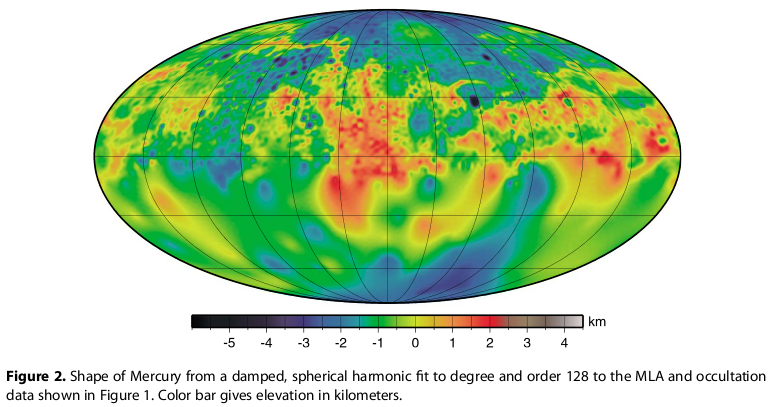
\includegraphics[scale=0.5]{MercuryMap.png}
\end{center}{
\footnotesize {\sc Figure 1.} Figure 2 from the Perry et al. (2015) paper: ``The Low-Degree Shape of Mercury''}
\label{fig:MercuryMap}
\end{figure}


\bibliographystyle{te}
\bibliography{bibl}


\end{document}
